% This text is proprietary.
% It's a part of presentation made by myself.
% It may not used commercial.
% The noncommercial use such as private and study is free
% Sep. 2005 
% Author: Sascha Frank 
% University Freiburg 
% www.informatik.uni-freiburg.de/~frank/
%
% additional usepackage{beamerthemeshadow} is used
%  
%  \beamersetuncovermixins{\opaqueness<1>{25}}{\opaqueness<2->{15}}
%  with this the elements which were coming soon were only hinted
%\documentclass[8pt]{beamer}
\documentclass[10pt]{beamer}
\usepackage{etex}
\newenvironment<>{varblock}[2][\textwidth]{%
  \setlength{\textwidth}{#1}
  \begin{actionenv}#3%
    \def\insertblocktitle{#2}%
    \par%
    \usebeamertemplate{block begin}}
  {\par%
    \usebeamertemplate{block end}%
  \end{actionenv}}
%\usepackage{hyperref}
%\usepackage{natbib}
%\usepackage{beamerthemeshadow}
\usepackage{beamerinnerthemecircles, beamerouterthemeshadow}

\usepackage{amsmath,amssymb,amsfonts}
\usepackage[pdf]{pstricks}
%\usepackage{bbm}
%\usepackage{booktabs}
\usepackage{amsthm}
\usepackage{booktabs}
\usepackage{graphicx}
\usepackage{epsfig}
%\usepackage{graphics}

% MQ: This is to be able to compile on the Riksbank computer. Uncomment with my laptop. Ugly solution but will have to do for now.
%\usepackage{epstopdf}
%\epstopdfsetup{outdir=./}

\usepackage{rotating}

\usepackage{url}
\usepackage{breqn}
%\usepackage{hyperref}
\usepackage[authoryear]{natbib}
\usepackage{setspace}
\usepackage{multirow}
%\usepackage{harvard}
\usepackage{xcolor}
%\usepackage{multicolumn}
\usepackage{algpseudocode}
\usepackage{sidecap}
\usepackage{bbm} 
\usepackage{courier}
\usepackage{tikz}
\usetikzlibrary{arrows,shapes,snakes,automata,backgrounds,petri}

\tikzset{
  treenode/.style = {align=center, inner sep=0pt, text centered,
    font=\sffamily},
  arn_n/.style = {treenode, circle, white, font=\sffamily\bfseries, draw=black,
    fill=black, text width=1.5em},% arbre rouge noir, noeud noir
  arn_r/.style = {treenode, circle, red, draw=red, 
    text width=1.5em, very thick},% arbre rouge noir, noeud rouge
  arn_x/.style = {treenode, rectangle, draw=black,
    minimum width=0.5em, minimum height=0.5em}% arbre rouge noir, nil
}
\beamertemplatenavigationsymbolsempty

\newenvironment{myenumerate}{\begin{enumerate}[(1)]}{\end{enumerate}} 
\sidecaptionvpos{figure}{c}
% FOR COLORING PARTS  OF TABLE
%\usepackage[beamer,customcolors]{hf-tikz}

%\tikzset{hl/.style={
%    set fill color=red!80!black!40,
%    set border color=red!80!black,
%  },
%}

\mode<presentation> {
    \usetheme{Madrid} %Frankfurt} %Bergen, Berkely, Berlin, Boadilla, CambridgeUS, Darmstadt,
                          %Frankfurt, Goettingen, Singapore, Warsaw
    \usecolortheme{beaver} %seahorse} %default} %beetle, seahorse, wolverine, dolphin, beaver
    %\useoutertheme[subsection=true]{smoothbars} 
    \usefonttheme{default}
    %\usecolortheme{red}
    

	\setbeamercolor{block title}{use=unstructure, fg=white, bg=purple!75!black} %{use=structure,fg=white,bg=purple!75!black}
	%\setbeamercolor{block body}{use=structure,fg=black,bg=white!20!white}    
    %\setbeamercolor{block body}{bg=white}
    \setbeamertemplate{enumerate items}[default]
    \setbeamercolor{enumerate item}{fg=purple!75!black} 
    \setbeamercolor{enumerate subitem}{fg=purple!75!black} 	 
	\setbeamercolor{itemize item}{fg=purple!75!black}  
	\setbeamertemplate{itemize item}[triangle]  
	\setbeamercolor{itemize subitem}{fg=purple!75!black}
	\setbeamertemplate{itemize subitem}[triangle]
	\setbeamertemplate{blocks}[framed]


}



%\usepackage{colortbl}
%\definecolor{yellow}{cmyk}{0,0.18,0.90,0.00}

%\usepackage{xcolor}

%\usepackage[authoryear]{natbib}
\begin{document}
\title[Lecture 10]{Bayesian Learning 732A46: Lecture 10}  
\author[Matias Quiroz]{Matias Quiroz\inst{1}$^{,}$\inst{2}}
\setbeamerfont{institute}{size=\fontsize{7pt}{8pt}}
\institute[LiU and Riksbank]{
  \inst{1}%
   Division of Statistics and Machine Learning, Link\"{o}ping University\\~\\
  \inst{2}%
   Research Division, Sveriges Riksbank\\
     
}

%\institute[Riksbank and LiU]{Sveriges Riksbank and Division of Statistics and Machine Learning, Link\"{o}ping University}

\date[]{May 2016} %\today 

%\usebackgroundtemplate{%
%  \vbox to \paperheight{\vfil\hbox to \paperwidth{\hfil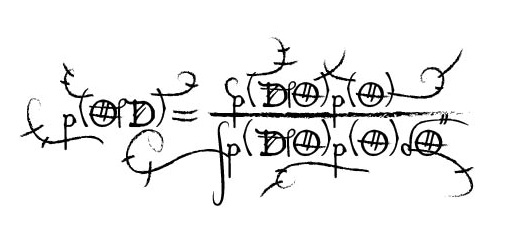
\includegraphics[width=1.5in]{Bayes.jpg}\hfil}\vfil}
%}

{
%\usebackgroundtemplate{\begin{center}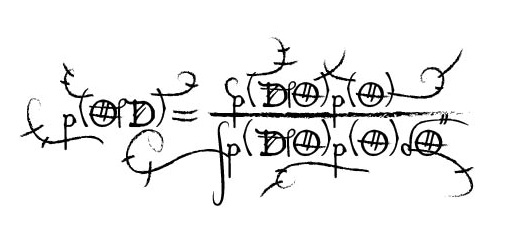
\includegraphics[width=0.4\paperwidth]{Bayes.jpg}\end{center}}
\usebackgroundtemplate{%
  \vbox to \paperheight{\hbox to \paperwidth{\hfil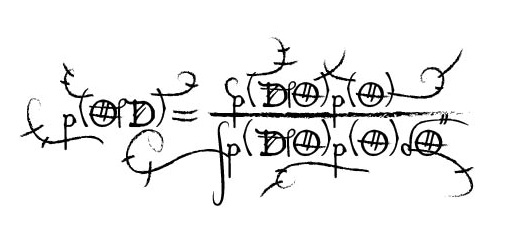
\includegraphics[width=2in]{Bayes.jpg}\hfil}}
}
\begin{frame}
\titlepage
\end{frame}
}
%\frame{\titlepage} 

%\frame{\frametitle{Overview of the talk}\tableofcontents}


\begin{frame}
\frametitle{Lecture overview}

\begin{itemize}
\item Bayesian model comparison
\bigskip
\item Computing marginal likelihoods
\bigskip
\item Bayesian model averaging

\end{itemize}

\end{frame}


\begin{frame}{Using the likelihood for model comparison}

\begin{itemize}
\item Consider two models for the data $y=(y_{1},...,y_{n})$:
$M_{1}$ and $M_{2}$.
\item Let $p_{k}(y|\theta_{k})$ denote the \textbf{\color{blue}data density} (fixed $\theta_k$) under
model $M_{k}$. %\medskip{}

\item If we know $\theta_{1}$ and $\theta_{2}$, the \textbf{likelihood ratio}
is useful 
\[
\frac{p_{1}(y|\theta_{1})}{p_{2}(y|\theta_{2})}.
\]
\item But often we \textbf{\color{red}do not know} $\theta_1$ and $\theta_2$.
\item \textbf{\color{blue}Frequentist}: The\textbf{\textcolor{blue}{{} likelihood ratio}} with the \textcolor{blue}{MLE} plugged in:
\[
\frac{p_{1}(y|\hat{\theta}_{1})}{p_{2}(y|\hat{\theta}_{2})}.
\]

\item \textbf{Bigger models} always win with estimated likelihood ratio.
\item \textbf{\textcolor{blue}{Hypothesis tests}} become problematic for non-nested
models.
\end{itemize}
\end{frame}

\begin{frame}{Bayesian model comparison}

\begin{itemize}
\item Use your priors $p_{1}(\theta_{1})$ and $p_{2}(\theta_{2})$ to get rid (\textbf{\color{blue}average over}) of $\theta$.
\item The\textcolor{blue}{{} }\textbf{\textcolor{blue}{marginal likelihood
}}for model $M_{k}$ with parameters $\theta_{k}$
\[
p_{k}(y)=\int p_{k}(y|\theta_{k})p_{k}(\theta_{k})d\theta_{k}.
\]
\item Recall \textbf{\color{blue}Bayes' theorem} in the simple case of $\theta = \{H, H^c\}$
$$\Pr(H|E)=\frac{\Pr(E|H)\Pr(H)}{\Pr(E)}, \quad \Pr(E) = \Pr(E|H)\Pr(H) + \Pr(E|H^{c})\Pr(H^{c})$$

\begin{center}
\begin{minipage}{\columnwidth}
\begin{varblock}[0.8\columnwidth]{\color{yellow}The marginal likelihood in words}
The \textbf{\color{blue}marginal likelihood} $\Pr(E)$ is a \textbf{\color{red}weighted average} of the probability of the evidence under the different hypothesis. The weights \textbf{\color{red}are given by the prior probabilities}.
\end{varblock}
\end{minipage}
\end{center}
\medskip
\item $\theta_{k}$ (or $H,H^c$) is removed (\textbf{\color{blue}averaged out}) by the prior. \textbf{\textcolor{red}{Priors matter!}}
\end{itemize}
\end{frame}



\begin{frame}{Bayesian model comparison, cont.}

\begin{itemize}
\item The \textbf{\textcolor{blue}{Bayes factor}}
\[
B_{12}(y)=\frac{p_{1}(y)}{p_{2}(y)}.
\]
\bigskip
\item \textbf{\textcolor{blue}{Bayesian machinery}}: Posterior model probabilities
\[
\underbrace{\Pr(M_{k}\vert y)}_{\text{Posterior model prob.}} \propto \underbrace{p(y\vert M_{k})}_{\text{marginal likelihood }[=p_k(y)]} \cdot \underbrace{\Pr(M_{k})}_{\text{prior model prob.}} 
\]
\bigskip
\item \textbf{\color{red}Important}: Two sets of priors
\begin{enumerate}
\item Prior for \textbf{\color{blue}the parameters} $\theta_{k}$ within model $M_{k}$ (\textbf{"the usual" prior})
\item Prior for \textbf{\color{blue}the models} $\Pr(M_{k})$.
\end{enumerate}
\end{itemize}
\end{frame}



\begin{frame}{Priors matter}

\begin{center}
%\includegraphics[width=0.5\columnwidth]{threePointPrior}\hspace{5mm}\includegraphics[width=0.45\columnwidth]{MargLike}
\includegraphics[scale=0.35]{threePointPrior}\hspace{1mm}\includegraphics[scale=0.35]{MargLike}

%\includegraphics[scale=0.35,bb = 0 0 200 100, draft, type=eps]{../../../Seminars/BayesLund2015/threePointPrior.eps}\includegraphics[scale=0.35,bb = 0 0 200 100, draft, type=eps]{../../../Seminars/BayesLund2015/MargLike.eps}
\par\end{center}

\end{frame}

\begin{frame}{Example: Geometric vs Poisson}

\begin{itemize}
\item Model 1 - \textbf{\textcolor{blue}{Geometric}} with \textbf{Beta} prior:

\begin{itemize}
\item $y_{1},...,y_{n}\vert\theta_{1}\sim \mathrm{Geometric}(\theta_{1})$, $$p(y_i|\theta_1)=(1-\theta_1)^{y_i}\theta_1 \quad	y_i \in \{0, 1, 2, \dots\}, 0 \leq \theta_1 \leq 1.$$
\item $\theta_{1}\sim \mathrm{Beta}(\alpha_{1},\beta_{1})$,
$$p(\theta_1)=\frac{\Gamma(\alpha_1 + \beta_1)}{\Gamma(\alpha_1)\Gamma(\beta_1)} \theta_1^{\alpha_1-1}(1-\theta_1)^{\beta_1 - 1}.$$
\end{itemize}
\bigskip
\item Model 2 - \textbf{\textcolor{blue}{Poisson}} with \textbf{Gamma} prior:
\begin{itemize}
\item $y_{1},...,y_{n}\vert\theta_{2}\sim \mathrm{Poisson}(\theta_{2})$, $$p(y_i|\theta_2)=\frac{\theta_2^{y_i}\exp(-\theta_2)}{y_i!} \quad	y_i \in \{0, 1, 2, \dots\}, \theta_2 > 0.$$
\item $\theta_{2}\sim \mathrm{Gamma}(\alpha_{2},\beta_{2})$, $$p(\theta_2)=\frac{\beta_2^{\alpha_2}}{\Gamma(\alpha_2)}\theta_2^{\alpha_2 - 1}\exp(-\beta_2 \theta_2).$$
\end{itemize}
\end{itemize}
\end{frame}



\begin{frame}{Geometric vs Poisson: $p(y)$ for Geometric ($M_{1}$)}

\begin{itemize}
\item \textbf{\color{blue}Marginal likelihood} for $M_{1}$ [$y = (y_1, \dots, y_n)$]
\begin{align*}
p_{1}(y) & =\int p_{1}(y\vert\theta_{1})p(\theta_{1})d\theta_{1}\\
 & = \int \left(\prod_{i=1}^n p(y_i\vert\theta_{1})\right) p(\theta_{1})d\theta_{1} \\
& = \frac{\Gamma(\alpha_1 + \beta_1)}{\Gamma(\alpha_1)\Gamma(\beta_1)}  \int (1-\theta_1)^{\sum_{i = 1}^n y_i} \theta_1^n \times \theta_1^{\alpha_1-1}(1-\theta_1)^{\beta_1 - 1} d\theta_1 \\
& = \frac{\Gamma(\alpha_1 + \beta_1)}{\Gamma(\alpha_1)\Gamma(\beta_1)}  \int \theta_1^{n + \alpha_1-1} (1-\theta_1)^{n \bar{y} + \beta_1 - 1}  d\theta_1\\ 
\end{align*}
\item The \textbf{\color{blue}beta function}
$$B(a, b) = \int_0^1 t^{a - 1}(1 - t)^{b - 1}dt, \quad a,b>0.$$ 
\item \textbf{Nice property} of the beta function
$$B(a, b) = \frac{\Gamma(a)\Gamma(b)}{\Gamma(a + b)}.$$

\end{itemize}
\end{frame}



\begin{frame}{Geometric vs Poisson: $p(y)$ for Geometric ($M_{1}$), cont}

\begin{itemize}
\item \textbf{\color{blue}Thus}
\begin{align*}
p_{1}(y) & =  \frac{\Gamma(\alpha_1 + \beta_1)}{\Gamma(\alpha_1)\Gamma(\beta_1)}  \int \theta_1^{n + \alpha_1-1} (1-\theta_1)^{n \bar{y} + \beta_1 - 1}  d\theta_1 \\
& =  \frac{\Gamma(\alpha_1 + \beta_1)}{\Gamma(\alpha_1)\Gamma(\beta_1)} B(n + \alpha_1, n \bar{y} + \beta_1) \\
& = \frac{\Gamma(\alpha_1 + \beta_1)}{\Gamma(\alpha_1)\Gamma(\beta_1)} \frac{\Gamma(n + \alpha_1)\Gamma(n \bar{y} + \beta_1)}{\Gamma(n + \alpha_1 + n \bar{y} + \beta_1)}.
\end{align*}
\item \textbf{\color{blue}Note}: It \textbf{\color{red}does not} depend on $\theta_1$. $\theta_1$ has been averaged out! 

\end{itemize}
\end{frame}


\begin{frame}{Geometric vs Poisson: $p(y)$ for Poisson ($M_{2}$)}

\begin{itemize}
\item \textbf{\color{blue}Marginal likelihood} for $M_{2}$ [$y = (y_1, \dots, y_n)$]
\begin{align*}
p_{2}(y) & =\int p_{2}(y\vert\theta_{2})p(\theta_{2})d\theta_{2}\\
 & = \int \left(\prod_{i=1}^n p(y_i\vert\theta_{2})\right) p(\theta_{2})d\theta_{2} \\
& = \frac{\beta_2^{\alpha_2}}{\Gamma(\alpha_2)} \int  \frac{\theta^{\sum y_i}_2}{\prod_{i=1}^n y_i}\exp(-n\theta_2) \times \theta_2^{\alpha_2 - 1}\exp(-\beta_2 \theta_2)d\theta_2 \\
& = \frac{\beta_2^{\alpha_2}}{\Gamma(\alpha_2)\prod_{i=1}^n y_i} \int  \theta_2^{n\bar{y}+\alpha_2 - 1}\exp(-(n+\beta_2) \theta_2) d\theta_2
\end{align*}
\item The \textbf{\color{blue}gamma function}
$$\Gamma(c) = \int_0^{\infty} t^{c - 1}\exp(-t)dt,\quad c>0.$$ 
\item ... rewritten to fit \textbf{our form above} (simple change of variables) ...
$$\frac{1}{(n+\beta_2)^c} \Gamma(c) = \int_0^{\infty} t^{c - 1}\exp(-(n + \beta_2)t)dt,\quad c>0.$$

\end{itemize}
\end{frame}


\begin{frame}{Geometric vs Poisson: $p(y)$ for Poisson ($M_{2}$), cont.}

\begin{itemize}
\item \textbf{\color{blue}Thus}
\begin{align*}
p_{2}(y) & = \frac{\beta_2^{\alpha_2}}{\Gamma(\alpha_2)\prod_{i=1}^n y_i} \int  \theta_2^{n\bar{y}+\alpha_2 - 1}\exp(-(n+\beta_2) \theta_2) d\theta_2 \\
& = \frac{\beta_2^{\alpha_2}\Gamma(n\bar{y} + \alpha_2 )}{\Gamma(\alpha_2) (n+\beta_2)^{n\bar{y} + \alpha_2} \prod_{i=1}^n y_i}.
\end{align*}
\bigskip
\item \textbf{\color{blue}Note} (\textbf{again!}): It \textbf{\color{red}does not} depend on $\theta_2$. $\theta_2$ has been averaged out!
\end{itemize}
\end{frame}

\begin{frame}{Geometric vs Poisson, cont.}

\begin{itemize}
\item \textbf{Before} comparing the results we need to set the hyper-parameters in \textbf{\color{blue}some suitable way}.\bigskip 
\item Set \textbf{\color{blue}hyper-parameters} so that the prior predictive means match 
\[
E(y_{i}\vert M_{1})=E(y_{i}\vert M_{2})\quad\Longrightarrow\quad (\alpha_{1} - 1) \alpha_{2}=\beta_{1}\beta_{2}
\]\bigskip
\item The \textbf{\color{blue}prior predictive mean} computed by the \textbf{\color{blue}tower property}
$$E(y_{i}\vert M_{k}) = E_\theta \left(E_{y_i | \theta}(y_{i}| \theta,M_{k})\right), \quad \text{for }k=1,2,$$
and $$E_{y_i | \theta}(y_{i}| \theta,M_{k})=\begin{cases}
\frac{\theta_1}{1-\theta_1},\text{ if } k=1\\
\theta_2,\text{~~~ if } k=2.
\end{cases}$$
\end{itemize}

\end{frame}



% Uncomment just for now
\begin{frame}{Geometric vs Poisson for Pois(1) data}


\begin{center}
\includegraphics[scale=0.5]{ConvergenceModelProbPoisData}
%\includegraphics[scale=0.5,bb = 0 0 200 100, draft, type=eps]{../../../Seminars/BayesLund2015/ConvergenceModelProbPoisData.eps}
\par\end{center}

\end{frame}

\begin{frame}{Geometric vs Poisson for Pois(1) data}


\begin{center}
\includegraphics[scale=0.5]{ConvergenceModelProbPoisDataLonger}
%\includegraphics[scale=0.5,bb = 0 0 200 100, draft, type=eps]{../../../Seminars/BayesLund2015/ConvergenceModelProbPoisDataLonger.eps}
\par\end{center}

\end{frame}

\begin{frame}{Properties of Bayesian model comparison}

\begin{itemize}
\item \textbf{\color{red}Coherence} of pair-wise comparisons
\[
B_{12}=B_{13}\cdot B_{32}.
\]

\item \textbf{\textcolor{red}{Consistency}} when true model is in $\mathcal{M}=\{M_{1},...,M_{K}\}$
\[
\mathrm{Pr}\left(M=M_{TRUE}\vert y \right)\rightarrow1\quad\text{as}\quad n\rightarrow\infty.
\]

\item \textbf{\color{red}``KL-consistency''} when $M_{TRUE}\notin\mathcal{M}$
\[
\mathrm{Pr}\left(M=M^{\star}\vert y\right)\rightarrow1\quad\text{as}\quad n\rightarrow\infty,
\]
where $M^{\star}$ is the model that minimizes Kullback-Leibler distance $$D_{KL}(p_{TRUE}, p_M) = \int p_{TRUE}(y) \log\left(\frac{p_M(y)}{p_{TRUE}(y)}\right) dy$$
between $p_{M}(y)$ and $p_{TRUE}(y)$.
\end{itemize}
\end{frame}


\begin{frame}{Some warnings}

\begin{itemize}
\item Smaller models \textbf{always win} when priors are very vague. 
\bigskip
\item \textbf{Improper priors} \textbf{\color{red}can't be used} for model comparison.
\bigskip
\item \textbf{\color{blue}Bayes factors} are \textbf{relative measures}! \textbf{\color{red}Does not} say anything about a single model's adequacy.

\end{itemize}
\end{frame}







\begin{frame}{Bayesian hypothesis testing}

\begin{itemize}
\item \textbf{\textcolor{blue}{Hypothesis testing}} is a \textbf{model selection} problem.
\item \textbf{Example}: Bernoulli model with prior $\theta \sim \mathrm{Beta}(\alpha, \beta)$ 
\begin{align*}
M_{0}:  y_{1},...,y_{n} | \theta_0 & \overset{iid}{\sim}\mathrm{Bernoulli}(\theta_{0})\\
M_{1}:  y_{1},...,y_{n}| \theta  & \overset{iid}{\sim}\mathrm{Bernoulli}(\theta).
\end{align*}
\item \textbf{\color{blue}Likelihood}: $p(y|\theta) = \theta^s (1-\theta)^f  $ ($y=(y_1, \dots, y_n)$, $s=\sum y_i$, $f = n - s$).
\item \textbf{\color{blue}Marginal likelihoods}
\begin{itemize}
\item For model $M_1$ $$p(y|M_1) = \theta^s (1-\theta)^f.$$
\item For model $M_2$ 
\begin{align*}
p(y|M_2) & = \int \theta^s (1-\theta)^f \frac{\Gamma(\alpha + \beta)}{\Gamma(\alpha)\Gamma(\beta)} \theta^{\alpha - 1} (1-\theta)^{\beta - 1} d\theta \\ 
& = \frac{\Gamma(\alpha + \beta)\Gamma(s + \alpha)\Gamma(f + \beta)}{\Gamma(\alpha)\Gamma(\beta)\Gamma(n + \alpha + \beta)}.
\end{align*}

\end{itemize}
\end{itemize}
\end{frame}


\begin{frame}{Bayesian hypothesis testing, cont.}

\begin{itemize}
\item Reject (or accept) based on the \textbf{\color{blue}posterior model probabilities}
\[
Pr(M_{k}|y)\propto p(y|M_{k})Pr(M_{k}),\text{ for }k=0,1.
\]
%\medskip
\item A \textbf{\color{red}"sharp null"} hypothesis is equivalent to using '\textbf{\textcolor{blue}{spike-and-slab}}' prior:
\[
p(\theta)=\pi \delta_{\theta_{0}}(\theta)+(1-\pi) \mathrm{Beta}(\alpha,\beta).
\]
%\bigskip
\item Think about the \textbf{\color{blue}shrinkage mechanism}! 
\bigskip
\item \textbf{\color{blue}Note}: data can now \textbf{\color{blue}support} a null hypothesis (not only reject
it). 

\end{itemize}
\end{frame}






\begin{frame}{Spike-and-slab prior [with $\theta_0 = 0.5$]}


\begin{center}
\includegraphics[scale=0.5]{spikeandslab}
%\textbf{\includegraphics[scale=0.5,bb = 0 0 200 100, draft, type=eps]{../../../Seminars/BayesLund2015/spikeandslab.eps}}
\par\end{center}

\end{frame}

\begin{frame}{Marginal likelihood - a measure of out-of-sample predictive performance}

\begin{itemize}
\item \textbf{\color{blue}The marginal likelihood} can be decomposed as
\[
p(y_{1},...,y_{n})=p(y_{1})p(y_{2}|y_{1})\cdots p(y_{n}|y_{1},y_{2},...,y_{n-1}).
\]
\item Assume that $y_{i}$ is \textbf{\color{red}independent} of $y_{1},...,y_{i-1}$
\textbf{\color{blue}conditional} on $\theta$:
\[
p(y_{i}|y_{1},...,y_{i-1})=\int p(y_{i}|\theta)p(\theta|y_{1},...,y_{i-1})d\theta
\]

\item \textbf{\color{blue}The prediction} of $y_{1}$ is \textbf{based on the prior} of $\theta$, and
is therefore \textbf{sensitive to the prior}.\medskip{}

\item In contrast, \textbf{\color{blue}the prediction} of $y_{n}$ \textbf{uses almost all the data} to infer $\theta$. If $n$ is large \textbf{\color{red}influence of prior is negligible} for $y_n$.
\medskip
\item \textbf{\color{blue}Summary}: "Early" out-of-sample predictions are more influenced by $p(\theta)$.
\end{itemize}
\end{frame}

\begin{frame}{Illustrating the sensitivity to the prior for early obs}

\begin{itemize}
\item \textbf{\color{blue}Model}: $y_{1},...,y_{n}\vert\theta\sim \mathcal{N}(\theta,\sigma^{2})$
with $\sigma^{2}$ \textbf{\color{red}known}. 
\item \textbf{\color{blue}Prior}: $\theta \sim \mathcal{N}(0,\kappa^{2}\sigma^{2})$ [for simplified expressions].
\item \textbf{\color{blue}Partial posterior} up to observation $i-1$ ($\mu_0 = 0$)
\[
\theta|y_{1},...,y_{i-1}\sim N\left[w_{i}(\kappa)\cdot\bar{y}_{i-1},\frac{\sigma^{2}}{i-1+\kappa^{-2}}\right]
\]
where $w_{i}(\kappa)=\frac{i-1}{i-1+\kappa^{-2}}$ [\textit{the usual weighted average story}].\smallskip
\item \textbf{\color{blue}Predictive density} for obs $i-1$ 
\begin{align*}
y_{i}|y_{1},...,y_{i-1} & \sim N\left[w_{i}(\kappa)\cdot\bar{y}_{i-1},\sigma^{2}\left(1+\frac{1}{i-1+\kappa^{-2}}\right)\right].
\end{align*}

\item \textbf{Terms with $i$ large}: $y_{i}|y_{1},...,y_{i-1}\overset{approx}{\sim}\mathcal{N}\left(\bar{y}_{i-1},\sigma^{2}\right)$,
\textbf{\color{red}not sensitive} to $\kappa$
\item For $i=1$, $y_{1}\sim \mathcal{N}\left[0,\sigma^{2}\left(1+\frac{1}{\kappa^{-2}}\right)\right]$
can be \textbf{\color{red}very sensitive} to $\kappa$.
\end{itemize}
\end{frame}



\begin{frame}{First observation is sensitive to $\kappa$}


\begin{center}
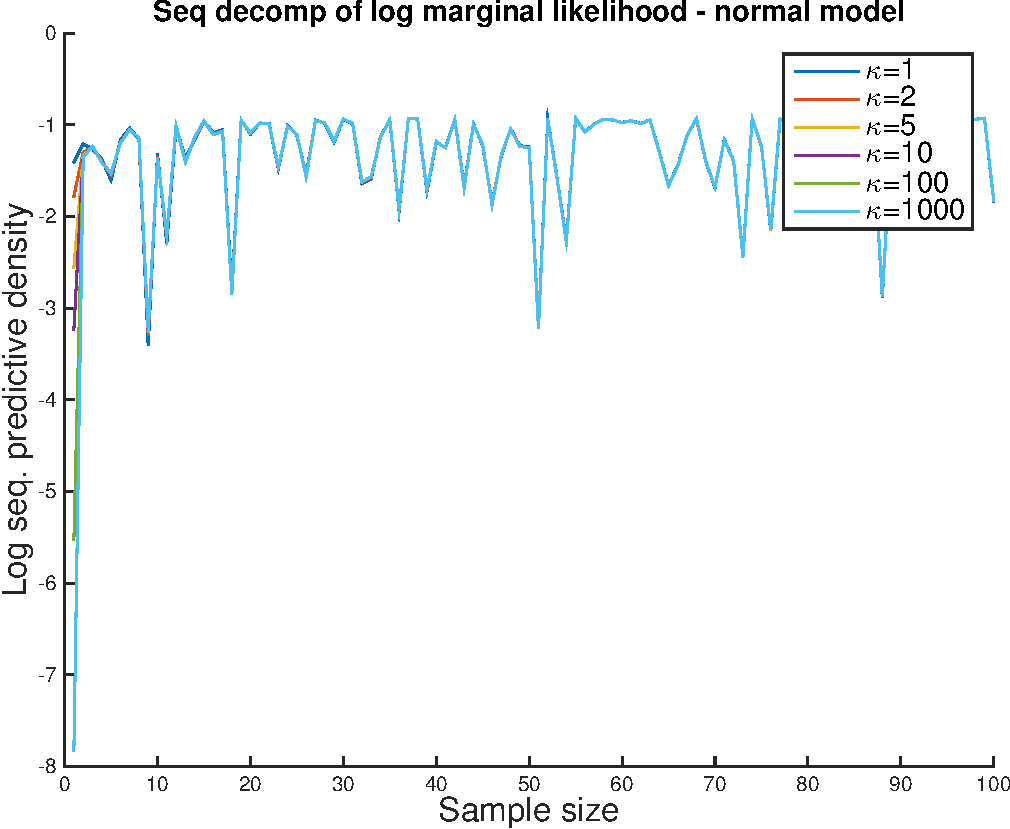
\includegraphics[scale=0.5]{SeqMargLikeNormal}
\par\end{center}

\end{frame}

\begin{frame}{First observation is sensitive to $\kappa$}


\begin{center}
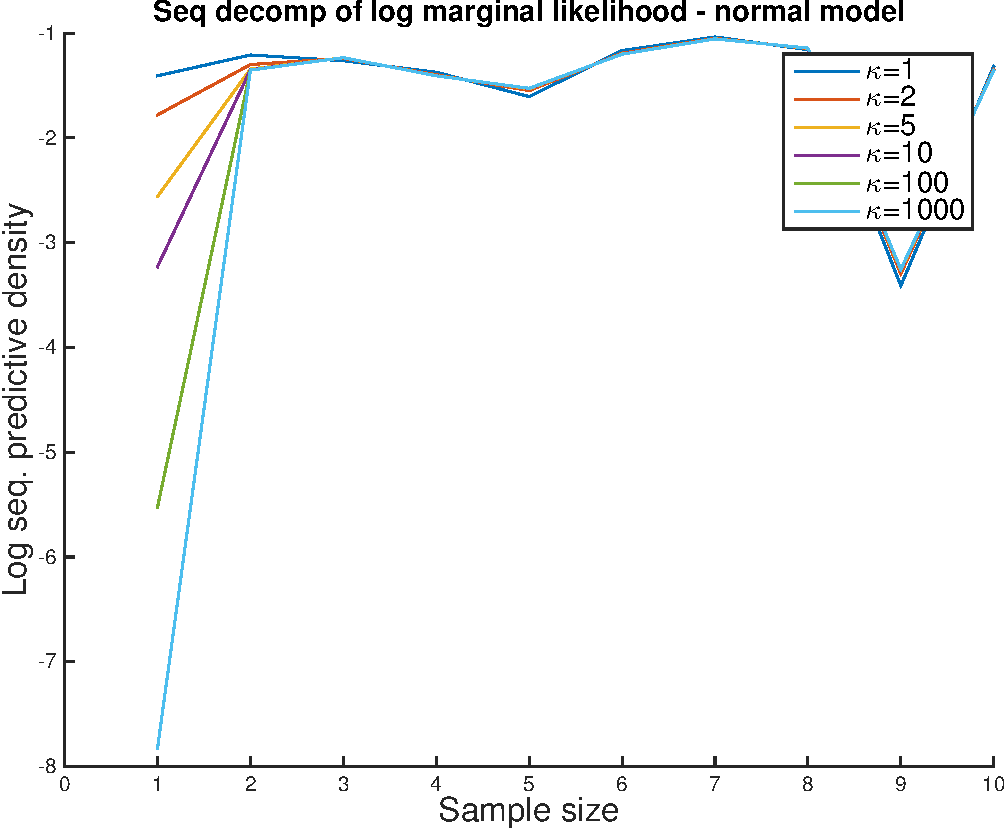
\includegraphics[scale=0.5]{SeqMargLikeNormalZoom}
\par\end{center}

\end{frame}

\begin{frame}{Log Predictive Score - LPS: a way to reduce the sensitivity}



\begin{itemize}
\item \textbf{Simple idea}: a measure similar to the marginal likelihood but where \textbf{\color{blue}the first observation is less sensitive} to the prior.
\item \textbf{Sacrifice}  $n^{\star}$ observations to train/update the prior.

\item \textbf{\color{blue}Predictive density score}: PS
\[
PS(n^{\star})=p(y_{n^{\star}+1}\vert y_{1},...,y_{n^{\star}})\cdots p(y_{n}\vert y_{1},...,y_{n-1}).
\]
\item \textbf{Compare} PS to $p(y)$ in factorized form.
\medskip{}
\item Usually report on log scale: \textbf{\textcolor{blue}{Log Predictive
Score}}\textcolor{blue}{{} }(\textbf{LPS}).\medskip{}

\item Which observations to \textbf{train/update} with (and which to predict)?\medskip{} 
\item \textbf{\color{blue}Split the data}: \textit{Training} and \textit{test} data 
\begin{itemize}
\item Straightforward for \textbf{time series}. %\medskip{}
\item \textbf{Cross-sectional data}: cross-validation is useful. 
\end{itemize} 

\end{itemize}
\end{frame}


\begin{frame}{Computing the marginal likelihood: Conjugate models}

\begin{itemize}
\item Computing the \textbf{\color{blue}marginal likelihood} requires integration w.r.t. $\theta$.\bigskip
\item \textbf{Short cut} for \textbf{\color{blue}conjugate models} by rearrangement of Bayes' theorem:
\[
p(y)=\frac{p(y|\theta)p(\theta)}{p(\theta|y)}.
\]
\medskip
\item By conjugacy $p(\theta|y)$ is \textbf{analytically available}.
\bigskip
\item Insert everything and \textbf{work out the algebra.}
\end{itemize}
\end{frame}

\begin{frame}{Computing the marginal likelihood: Simulation methods}

\begin{itemize}
\item Usually difficult (or \textbf{\color{red}impossible}) to analytically derive
\[
p(y)=\int p(y|\theta)p(\theta)d\theta=E_{\theta}[p(y|\theta)].
\]
\item Draw from the prior $\theta^{(1)},...,\theta^{(N)}$ and use the usual \textbf{\color{blue}Monte Carlo estimate}
\[
\hat{p}(y)=\frac{1}{N}\sum_{i=1}^{N}p(y|\theta^{(i)}).
\]
\item \textbf{\color{red}Unstable} (huge variance) if the likelihood is somewhat different from the prior.
\item \textbf{\textcolor{blue}{Importance sampling}}. Let $\theta^{(1)},...,\theta^{(N)}$
be iid draws from $g(\theta)$.
\[
\int p(y|\theta)p(\theta)d\theta=\int\frac{p(y|\theta)p(\theta)}{g(\theta)}g(\theta)d\theta\approx \frac{1}{N}\sum_{i=1}^{N}\frac{p(y|\theta^{(i)})p(\theta^{(i)})}{g(\theta^{(i)})}.
\]
 
\item \textbf{\textcolor{blue}{Modified Harmonic mean}}: $g(\theta)=\mathcal{N}(\tilde{\theta},\tilde{\Sigma})\cdot I_{c}(\theta)$,
where $\tilde{\theta}$ and $\tilde{\Sigma}$ is the posterior mean
and covariance matrix estimated from an MCMC chain, and $I_{c}(\theta)=1$
if $(\theta-\tilde{\theta})'\tilde{\Sigma}^{-1}(\theta-\tilde{\theta})\leq c$.
\end{itemize}
\end{frame}

\begin{frame}{Computing the marginal likelihood: Simulation methods, cont.}

\begin{itemize}
\item Rearrangement of \textbf{\color{blue}Bayes' theorem} (again!): $p(y)=p(y|\theta)p(\theta)/p(\theta|y)$.\medskip
\item \textbf{\color{blue}Note 1}: Need the full expression for the posterior, \textbf{including} the constants ind of $\theta$. \medskip{}
\item \textbf{\color{blue}Note 2}: LHS is \textbf{independent} of $\theta$. RHS \textbf{depends} on $\theta$... \medskip{}
\item ... any $\theta$ must cancel. Enough to evaluate in a single point $\theta_{0}$.\medskip{}
\item \textbf{Kernel density estimator} to approximate $p(\theta_{0}|y)$. Unstable. \medskip{}
\item Chib (1995) provide better solutions for \textbf{\color{blue}Gibbs sampling}.
\medskip{}
\item Chib and Jeliazkov (2001) generalizes to \textbf{\color{blue}MH algorithm} (good
for Independence MH, not so good for RWM).
\end{itemize}
\end{frame}

\begin{frame}{Computing the marginal likelihood: Approximation}

\begin{itemize}
\item By \textbf{normal approximation} of the posterior distribution (\textbf{\color{blue}Lecture 6}).\smallskip
\item \textbf{\color{blue}Recall}: for large $n$ 
\begin{align*}
p(\theta|y) & \approx \mathcal{N}_p(\theta^{\star}, \Sigma_{\theta^{\star}}=J^{-1}_{\theta^{\star}, y})\\
& = (2\pi)^{-p/2}|J^{-1}_{\theta^{\star}, y}|^{-1/2}\exp\left(-\frac{1}{2}(\theta-\theta^{\star})^{\prime}J_{\theta^{\star}, y}(\theta-\theta^{\star})\right).
\end{align*}
\item \textbf{\textcolor{blue}{The Laplace approximation}}: Use rearranged Bayes' theorem with $\theta=\theta^{\star}$
\[
\log\hat{p}(y)=\log p(y|\theta^{\star})+\log p(\theta^{\star})+\frac{p}{2}\log(2\pi)+\frac{1}{2}\log\left\vert J^{-1}_{\theta^{\star}, y}\right\vert.
\]
\item \textbf{\color{red}As usual}: $\theta^{\star}$ and $J_{\theta^{\star},y}$ [$-H_{\theta^{\star}}]$ are obtained via a numerical optimization (e.g. \texttt{optim} in \texttt{R}).


\end{itemize}
\end{frame}



\begin{frame}{Bayesian model averaging}

\begin{itemize}
\item Let $\gamma$ have the \textbf{same interpretation} across the model space
$$\mathcal{M} = \{M_1, \dots, M_K\}.$$
Let $\theta = \{\theta_1, \dots, \theta_K\}$ be the corresponding set of parameters.\medskip{}

\item The \textbf{\color{blue}marginal posterior} (marginalized over $\mathcal{M}$) of $\gamma$
\[
p(\gamma|y)=\int p(\gamma, \mathcal{M}|y)d\mathcal{M}=\sum_{k=1}^K p(\gamma|M_k, y) p(M_{k}|y),
\]
where $p(\gamma|M_k,y)$ is the \textbf{\color{blue}marginal posterior} (marginalized over $\theta_k$) of $\gamma$
conditional on model $k$, 
$$p(\gamma|M_k,y)=\int p(\gamma|\theta_k,y)p(\theta_k|y)d\theta_k.$$
\item Note the \textbf{\color{red}two layers} of averaging... \textbf{\color{red}Bayes is all about averaging out (marginalize) unknown quantities!}

\end{itemize}
\end{frame}


\begin{frame}{Bayesian model averaging, cont.}

\begin{itemize}
\item \textbf{\color{blue}Example}: $h$-step ahead prediction for time series: $\gamma=(y_{T+1},...,y_{T+h})$,
%\bigskip
\begin{align*}
p(\gamma|M_k,y) & = p_k(y_{T+1},...,y_{T+h}|y) \quad [\text{Posterior predictive for }M_k] \\
p(M_k | y) & \propto p(y|M_k)p(M_k), \quad [p(y|M_k) \text{ - Marg. likelihood for }M_k]
\end{align*}
\item $p(y_{T+1},...,y_{T+h}|y)$ includes \textbf{\textcolor{blue}{\color{red}three sources
of uncertainty}}:\medskip
\begin{itemize}
\item \textbf{\textcolor{blue}{Future errors}}/disturbances. \textbf{\color{blue}Simpler analogy}: $\sigma^2$ (assume known) in  \begin{align*}
y_1,\dots, y_n | \theta & \overset{iid}{\sim} \mathcal{N}(\theta,\sigma^2), \quad \text{and } p(\theta) \propto c \text{ gives}\\
p(\theta|y) & = \mathcal{N}(\bar{y},\sigma^2/n)  \\
p(\tilde{y}|y) & = \mathcal{N}\left(\bar{y},\sigma^2 + \frac{\sigma^2}{n}\right) \quad [\text{Posterior predictive for future } \tilde{y}].
\end{align*}
\item \textbf{\textcolor{blue}{Parameter uncertainty}} (Posterior predictive averaged over posterior of $\theta$).
\smallskip
\item \textbf{\textcolor{blue}{Model uncertainty}} (by model averaging).
\end{itemize}
\smallskip
\item \textbf{Any painful integrals}? Compute by simulation!


\end{itemize}
\end{frame}



\begin{frame}
\frametitle{References}

\small{
\textbf{Chib, S., (1995)}. Marginal likelihood from the Gibbs output. \textit{Journal of the American Statistical Association}, 90(432):1313-1321}
\\~\\
\small{
\textbf{Chib, S. and Jeliazkov, I. (2001)}. Marginal likelihood from the Metropolis–Hastings output. \textit{Journal of the American Statistical Association}, 96(453):270-281.}
\\~\\
\small{
\textbf{Lavine, M. and Schervish, M.J., (1999)}. Bayes factors: what they are and what they are not. \textit{The American Statistician}, 53(2):119-122.}

\end{frame}












\end{document}

